% Kapitel 7
%-------------------------------------------------------------------------------


\chapter{Benutzeroberfläche}

Die Benutzeroberfläche wird unterteilt in mindestens drei Webseiten:
Ausgehend von einer Suchseite, werden die Ergebnisse tabellarisch unter der
Suchmaske angezeigt, die auf Detailseiten weiterführen. 
Der Benutzer hat je nach Rechtestatus eine Gast-/Benutzer- oder eine Administrationsumgebung (zum Beispiel zum normalen Einsehen, Verändern, Löschen von Komponenten). 

\section{/B10/ Seitenlayout}

 \begin{itemize}
   \item Komponentendatenbank
   \begin{itemize}
    \item Suche
      \begin{description}
       \item[Einfache Suche] Die einfache Suche soll relativ unkompliziert funktionieren:
        Sie besteht lediglich aus einer Eingabefläche, worin der Benutzer
       den Namen der Komponente, Autoren oder Sonstiges eingeben kann. 
       \item[Erweiterte Suche] Die erweiterte Suche stellt mehrere Optionen zur Verfügung, um die Suche zu präzisieren. 
       \end{description}
    \end{itemize}
    \item Komponentenliste
    \item Login/Account
    \item Administration
 \end{itemize}
 
\begin{figure}
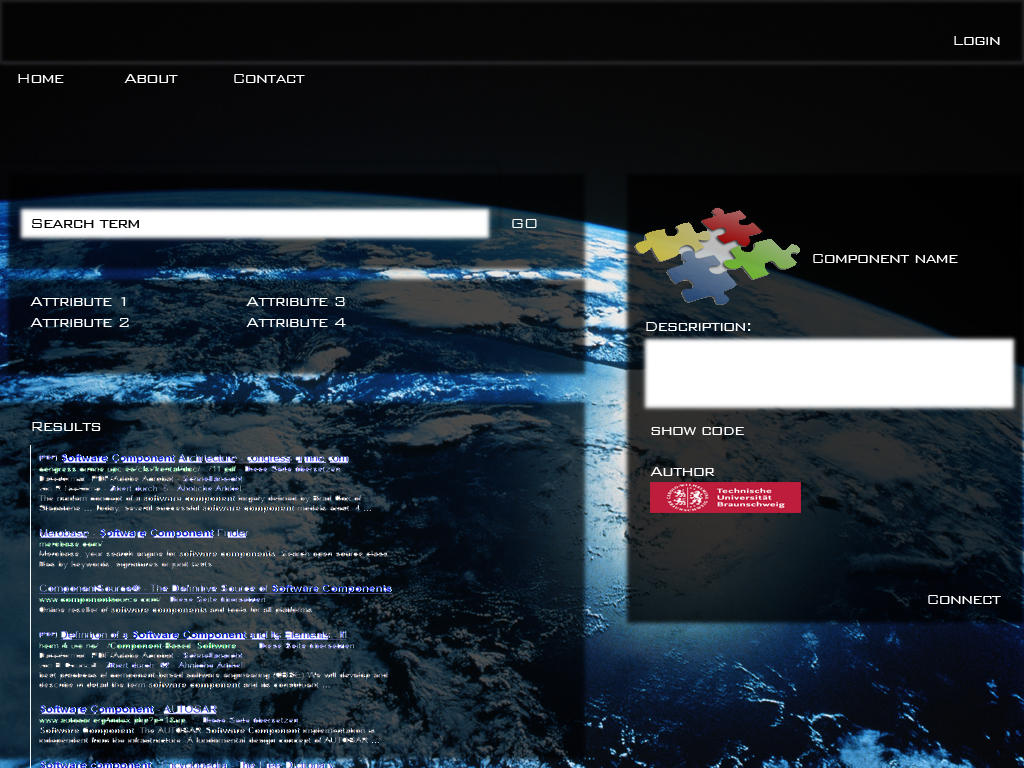
\includegraphics[width=0.8\linewidth]{bilder/overview.jpg}
\caption{Beispiel für ein Seitenlayout}
\label{fig:gui}
\end{figure}

Suchergebnisse werden in einem großen Bereich rechts bzw.\ unter der Navigation angezeigt. 
Die Komponenten werden übersichtlich in tabellenartiger Form bereitgestellt. Bei einem Klick auf ein bestimmtes Suchergebnisses erscheinen genauere Informationen über die Komponente. 
Oben rechts wird zudem der eingeloggte User angezeigt.
Bei einem Klick auf den eingeloggten User ist eine Account-Verwaltungsseite geplant.
